\chapter{SegMatch}
\label{chap:segmatch}

\section{Intro \& Pipeline}
\label{sec:intro-pipeline}
%TODO
The SegMatch algorithm is constituted of 5 main steps, data input, segmentation, description, matching, and geometric filtering. These 5 steps are illustrated in the usual SegMatch pipeline, as shown in Fig.~\ref{fig:pipeline}.\\

\begin{figure}
  \centering
  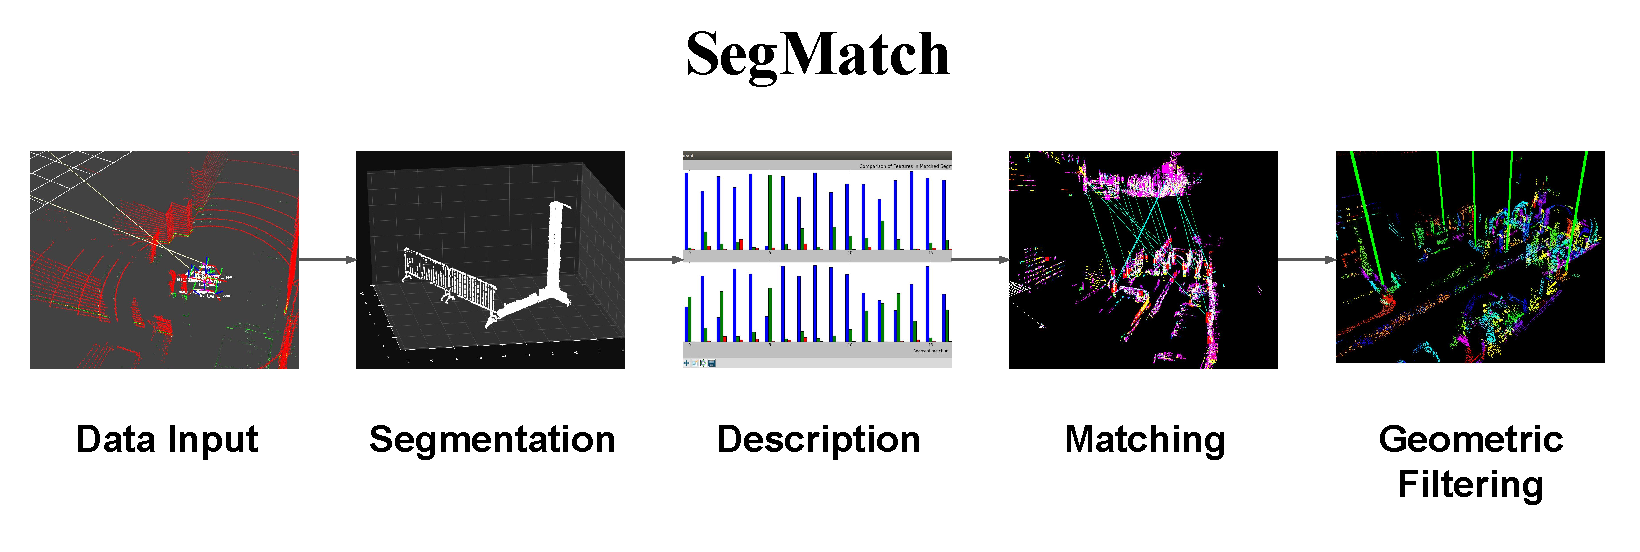
\includegraphics[width=5.2in]{images/pipeline.pdf}
  \caption{The SegMatch pipeline}
  \label{fig:pipeline}
\end{figure}

SegMatch can be used in a variety of situations where place recognition from range data is useful. Though the usual SegMatch algorithm (Fig.~\ref{fig:pipeline}) remains applicable to all such situations, there can be differences in how SegMatch should be integrated to the general pipeline, to interact with other robot or computer processes. Examples pipelines are given in Figures~\ref{fig:online_pipeline}, ~\ref{fig:offline_pipeline}, and ~\ref{fig:multirobot_pipeline} to showcase various uses of the SegMatch algorithm.

\begin{figure}
  \centering
  \includegraphics[width=5.2in]{images/Online Pipeline.pdf}
  \caption{An example of a simplified pipeline for using SegMatch online.}
  \label{fig:online_pipeline}
\end{figure}

\begin{figure}
  \centering
  \includegraphics[width=5.2in]{images/Offline Pipeline.pdf}
  \caption{An example of a simplified pipeline for using SegMatch offline.}
  \label{fig:offline_pipeline}
\end{figure}

\begin{figure}
  \centering
  \includegraphics[width=5.2in]{images/Multi-Robot Pipeline.pdf}
  \caption{An example of a simplified pipeline for using SegMatch online when several robots are exploring the same environment.}
  \label{fig:multirobot_pipeline}
\end{figure}

\section{Input}
\label{sec:input}

The first step of SegMatch is to acquire data on which the algorithm is performed. Segmatch takes as input two point clouds, the source and target, between which it attempts to find segment matches.\\

It sometimes happen that the target input is already segmented and described (see Section \ref{sec:online}), in which case the Segmentation and Description steps are only applied to the source cloud.\\

In any case, the Segmentation and Description steps are performed identically whether their input is the source or target cloud.\\

Usually, LiDAR sensors do not produce ready-made point clouds of the local area, and it may be necessary to consider this section's next subsections, \ref{subsec:sensordata}, \ref{subsec:distortion}, \ref{subsec:artefacts}, and \ref{subsec:SLAM}, to understand how raw sensor data can be transformed into SegMatch input.

\subsection{Sensor Data}
\label{subsec:sensordata}

Two types of sensors were used in the course of this project, rotating sensors (Velodyne) and rolling sensors (SICK). \\

Rotating sensors have a 360° view. With each rotation, they scan points along a cone originating from the sensor, resulting in a single circular scan line. This cone angle is varied by a set amount after each full rotation, with a maximum absolute angle making it so that the sensor is unable to scan the area directly above or under it. A typical rotating sensor scan is illustrated in Fig.~\ref{fig:velodyne-scan}.\\ % TODO

Rolling sensors have a 180° view, scanning towards the front and sides. The scan is flat, meaning that the points are all located on the same plane relative to the sensor’s roll angle. By varying this roll angle with every subsequent scan, the sensor can produce points at many vertical angles towards its sides. A typical rolling sensor scan is illustrated in Fig.~\ref{fig:sick-scan}.\\ % TODO

\subsection{Data Distortion}
\label{subsec:distortion}

As the sensor scans its surroundings, the robot may move and rotate. An extremum example: should the robot counter-rotate at the same angular velocity as its rotating-scanner, all points will be located on the same vertical plane in the world frame.\\

Naively mapping the full scan from sensor frame to world frame with a single affine transform will not accurately portray this effect. This is because each point was taken at a different point in time, and thus each has its own frame relative to the world frame - as the sensor was continually moving.\\

Precise knowledge of the robot’s odometry at various times during the scanning process allows to correct for distortion, by associating a different affine mapping from sensor frame to world frame to each group of points taken at a discrete rotation angle of the sensor.\\

In the case of rotating sensors, Philipp Kruesi has built the velodyne-assembler package \ref{velodyne-assembler} which corrects distortion in the aforementioned manner.\\ %TODO velodyne-assembler?

\subsection{Sensor Artefacts}
\label{subsec:artefacts}

After being corrected for distortion, sensor data contains registration patterns, as visible in Fig.~\ref{fig:velodyne-scan} (in this case, scan lines due to the rotating sensor's registration mechanics).

\subsection{Laser SLAM}
\label{subsec:SLAM}

As single sensor scans contain registration patterns (Subsection ~\ref{subsec:artefacts}), subsequent scans should be accumulated while the robot and sensor move, in order to collect data over the whole environment. Should the scans be assembled correctly, i.e, according to the correct transform w.r.t. each other, registration patterns get progressively reduced, as the accumulated data densifies.\\

To do so, knowledge of the robot's position and orientation at each sensor aquisition time is required. When the robot odometry is not sufficiently trustworthy, the Laser SLAM algorithm allows using the sensor data to increase the odometry knowledge and improve the quality of the accumulated data.\\

\section{Segmentation}
\label{sec:segmentation}

The process of segmentation consists in clustering points which share a common property. In our case, the goal is for that property to be appartenance to a particular object, in the real-world space equivalent to point-cloud space.\\

The input of this step is a 3D point cloud. If both source and target clouds are to be segmented, this step is imply applied once to the source and once to the target, in exactly the same way.

A perfect segmentation is however not explicitely defined. Should the point-cloud of a building be segmented into more basic components, such as walls, windows, and doors, or as single large cluster? Should a tree be clustered as a trunk with clusters of leaves above it or as a single cluster (illustrated in Fig.~\ref{fig:hierarchical})?\\

Moosman \cite{moosmann2011unsupervised} mentions hierarchically segmenting the scene, i.e., not only clustering point clouds into segments, but also subsegments and subsubsegments. As a result, a single point can be assigned to a segment, \textit{and} one of its subsegments, and so on. This segment hierarchy is established in order to capture those patterns that exist in real-world objects, which can be composed of smaller, simpler objects.\\

\begin{figure}
  \centering
  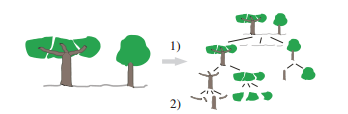
\includegraphics[width=3.2in]{images/hierarchical.png}
  \caption{Illustration of the hierarchical segmentation concept, by Moosman \cite{moosmann2011unsupervised}}
  \label{fig:hierarchical}
\end{figure}

It is useful to be aware of this concept of segment hierarchy even when using straightforward segmentation methods. \textit{Straightforward}, in this context, refers to segmentation algorithms which assign each point to at most one segment, and do not consider sub- and subsub- (etc \ldots) segments. Awareness of this hierarchy allows us to reason on where along it our segmentation algorithm works, and how that relates to the usefulness of the segments it produces.\\

For example, a specific algorithm, using a certain set of parameters, could tend to find segments which are very low in the hierarchy, i.e, smaller, less complex segments. This gives us a larger number of less unique segments, than say, running the same algorithm at a different scale.\\

By understanding this, it is easier to select the parameters which lead to optimal size, number and complexity of segments for the purposes of one's own use-case.\\

In this section, we present the main segmentation algorithms implemented and used in SegMatch. Their output and performance is discussed.\\

\subsection{Euclidean Clustering}
\label{subsec:euclidean}
%TODO

Euclidean clustering is the simplest segmentation method presented here. It consists in clustering together points which fall below a certain distance threshold $\delta$ from each other.\\

It is outlined by Douillard et Al. \cite{douillard2011segmentation} as the 'Cluster-All Method' of segmentation.\\

In terms of performance, the algorithm is very fast, allowing SegMatch to perform segmentation in real-time even on the fastest moving KITTI \cite{KITTI} datasets. This is due to the algorithm's simplicity.\\

On the other hand, we often see large objects getting segmented as single clusters, and smaller objects getting clustered together simply because they happen to lie close to each other.\\

Finally, it is generally necessary to filter out the ground as it tends to connect many objects together. This can offload complexity to ground filtering in the case of complex ground geometry, but is relatively simple to do in the case of a flat city street.\\

Parameters: Euclidean distance threshold.

\subsection{Difference of Normals Segmentation}
\label{subsec:DoN}
%TODO

Ioannou \cite{ioannou2012difference} presents the Difference of Normals segmentation algorithm, which aims to filter out geometrically uninteresting sections of the environment.\\

In order to do this, a difference of normals operator is defined, describing the variation in orientation with respect to scale, in the neighbouring environment. An illustration of this operator is shown in Fig.~\ref{fig:DoN}.\\

\begin{figure}
  \centering
  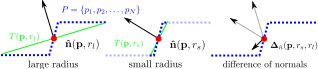
\includegraphics[width=3.2in]{images/DoN.png}
  \caption{The DoN operator according to Ioannou \cite{ioannou2012difference}}
  \label{fig:hierarchical}
\end{figure}

The average neighboring normals are first calculated at each point for neighbours which fall in a large scale radius $r_l$, then again for neighbours which fall in a small scale radius $r_s$. This process is often computationally heavy, increasingly so as the large scale increases (if nearest neighbours are not sampled).\\

For each point, a difference of normals is calculated between the average neighbour normals for the two scales. As a result, areas which are flat at both the large and small scale have a low difference of normals. Those points are filtered out, and the remaining points are clustered together if their DoN operators are similar.\\

Parameters: $r_s$, $r_l$, $\Delta_n^{threshold}$

\subsection{Region Growing}
\label{subsec:region-growing}

The Region Growing algorithm is notably useful for segmenting areas where curvature remains under a certain threshold.
%TODO

Parameters: $\theta$

\subsection{Optimizations}
\label{subsec:optimizations}
%TODO

D2Depth-based Segmentation\\
Normals from original scan

\section{Description}
\label{sec:description}

Descriptors allow us to compress information about each segment's properties into an n-dimensional feature vector.\\

The input to this step is a list of segments. The output is a n-dimensional feature vector, a \textit{description}, for each segment. Like the segmentation step, this step is applied once to source and once to target data.

An ideal descriptor would yield identical feature vectors for any segments which are views of the same real-world object. If two segments represent views of different objects their feature vectors should differ.\\

In other words, ideal descriptors lead to strong clustering in the n-dimensional feature space of segments representing views of the same objects. \\

A good descriptor is a descriptor which approaches this behavior, where segments which are views of the same object are often clustered close to each other. Weaker larger-scale clustering in accordance with object classes (objects that are similar yet not identical) can reasonably be expected.\\

This section outlines the pre-existing segment description algorithms used in SegMatch. In Chapter \ref{sec:segmatchAE}, we introduce our own descriptor based on an unsupervised learning approach.\\

\subsection{Eigenvalue-based Features}
\label{subsec:eigenvalues}

$\lambda_1$, $\lambda_2$, $\lambda_3$ are the eigenvalues of the covariance matrix $C \in \mathbb{R}^{3x3}$
$$
C = 
\begin{bmatrix}
  cov(\textbf{x},\textbf{x}) & cov(\textbf{y},\textbf{x}) & cov(\textbf{z},\textbf{x})  \\
  cov(\textbf{x},\textbf{y}) & cov(\textbf{y},\textbf{y}) & cov(\textbf{z},\textbf{y})  \\
  cov(\textbf{x},\textbf{z}) & cov(\textbf{y},\textbf{z}) & cov(\textbf{z},\textbf{z})  \\
\end{bmatrix} 
$$
$\textbf{x}$, $\textbf{y}$, $\textbf{z}$ being the coordinates of all points inside the segment.

\subsection{Ensemble of Shapes}
\label{subsec:ensemble-of-shapes}

This descriptor calculates the statistical measure of some properties for randomly selected point pairs/triplets within the object.\\
%TODO

\section{Matching}
\label{sec:matching}

Once descriptions of all source and target segments have been computed, the matching step is responsible for finding potential pairwise matches between source and target segments.\\ 

The inputs are one list of source segment descriptions, and one list of target segment descriptions. This step then outputs a list of potential matches between source and target segments based on their descriptions.\\

\subsection{kNN}
\label{subsec:kNN}

The simplest matching algorithm considered here, kNN selects the k nearest neighbours according to euclidean distances of a segment description in n-dimensional feature space.\\

In the case of an ideal descriptor, this algorithm is sufficient to recognize true segment matches, even with $k = 1$. As we recall, an ideal descriptor would ensure that all segments taken from a single object in the real world have identical features.\\ 

For sufficiently good descriptors, this algorithm can also be adequate, predicting mostly true matches and some false matches. One issue with descriptors that are not ideal is that they might not allow to distinguish precisely between objects in the same class.

That is, segments of the class 'car' might be clustered together, with small variation in their descriptors being tied to viewpoints or the area of a car that the segment covers, rather than idiosyncracies in the cars themselves. In this case it can be useful to increase $k$.\\

A common alternative to limiting the number of nearest neighbours with a threshold k, is to limit the nearest neighbours to all that fall within a certain threshold radius $r$. Furthermore, both thresholds can be combined, in order to limit nearest neighbours in both amount and distance.\\

It should be mentioned that the density of description clusters in n-dimensional space is not constant with some descriptors. In those cases, distance in n-dimensional space does not generalize well as a measure of similarity. To illustrate, for some descriptors, the same threshold radius can be very strict (i.e., containing many neighbours however dissimilar) in some regions of n-dimensional space, and not strict at all (i.e., filtering out all neighbours including desired ones) in others.\\

For descriptors which are further from the ideal, better matching results can be obtained by using a more complex matching algorithm than kNN.

\subsection{Random Forests}
\label{subsec:RF}

Random Forests are a Machine Learning algorithm which trains many decision trees simultaneously, then polls them in order to classify input.\\

In our case, the input is a pair of feature vectors belonging to two segments, and the output a boolean describing wether or not they are a match. This output can also instead be a probability of match $p$, with $0 \leq p \leq 1$.

%TODO

\section{Finding Patterns}
\label{sec:filtering}

%TODO
An efficient method to extract patterns of matches from a list of potential matches is the Geometric Consistency algorithm \cite{geometric-consistency}.\\

In this algorithm, matches are clustered together if they can form an Euclidean transformation, within a spatial tolerance $r$. As the Euclidean transformation has 6 degrees of freedom, any clusters with less than 3 matches is filtered out.\\

The clusters which remain, those consistuting of 3 or more matches, are loop closure candidates. The algorithm also returns the transformations formed by each of these clusters.\\

\section{Applying SegMatch - Online Example}
\label{sec:online}

Thus far into this chapter, the usual steps of the SegMatch algorithm have been presented. SegMatch can be applied to several situations, as outlined in Section \ref{sec:intro-pipeline}, without needing to modify any of the steps in the above sections.\\

What does change between implementations is \textit{when} to run SegMatch, \textit{what data} is to be taken as input, and of course the parameters.\\

The present section illustrates an example of how we applied SegMatch, in the case of a full online loop-closure-finding module in ROS.

\subsection{Segmentation Strategy}
\label{subsec:segmentation-strategy}

In the online scenario, the goal is to use SegMatch as-we-go in order to attempt to find matches between the most recent environment, and the recorded past environment.\\

As such, the overall process is to:   

\begin{enumerate}
\item Decide on the next instant or location at which to run SegMatch, and wait until it is reached.
\item Run SegMatch between the current local map and recorded past.
\item Add resulting segments to the recorded past.
\end{enumerate}

\subsection{Segmentation Frequency}
\label{subsec:segmentation-frequency}

The process of segmenting point clouds is one of the more computationally heavy parts of the pipeline. This motivates the development of a well-designed segmentation strategy - that is, a process driving the decision such as which areas of the observed cloud to store, send for segmentation, and when.\\

Regarding time: it is intuited that regions of space should be passed through the segmenter when they are most accurate and dense. This presents a trade-off problem. The longer one waits before segmenting, the worse positioning confidence is, and the larger the uncertainty in the points' fixed frame position (this leads to 'fuzzy' segments).\\

Not waiting long enough, on the other hand, leads to sparse segments, which might be missing important geometrical information, or introduce artefacts - such as scan-line patterns.

One way of handling this trade-off is to set a target `sufficient density', where it is estimated that increasing density leads to diminishing information gain.\\

From that point on, the costs of increasing density - i.e. loss of accuracy - outweigh the benefits, and segmentation should be undertaken.\\

During the accumulative process of capturing a point cloud map, the sensor might cover regions which will reach this sufficient density at different times.

Within this paradigm, it would be optimal to segment different areas at different times even though they were captured simultaneously.\\


This leads to quite complicated algorithms, and increases the amount of parameters which need to be tuned.\\

However, though far away objects densify more slowly, they accumulate positional uncertainty faster. They are also less useful for positioning and place recognition, due to parallax effects.\\

Thus it can be advantageous to prioritize closer objects, which allows one to assume a single rate of density increase for the whole area being captured - fixed to the close objects densification rate.\\

The resulting strategy is excessively simple: accumulate all points, until target density is reached in nearby objects, then segment all accumulated points. After segmentation, discard those points and start over.\\

A further idealization is to relate densification to movement. This is particularly true of rotating LIDAR systems such as the velodyne, with wich the sensor can only cover new areas if the robot moves.\\

According to this idealization, when the robot has moved a certain amount $\Delta x$ it densifies nearby objects by the amount $\Delta D$.

Assuming that the relationship between the two can be modelled with a simple proportionality,
$$\frac{\Delta x}{\Delta D} = \alpha$$
we are able to conclude that target density is reached when
$$x_{target} = D_{target} * \alpha$$
which gives us a simple rule: Segment the cloud every time the robot has moved/rotated by a certain amount $x_{target}$.\\

Based on the range of the velodyne sensor, this density $D_{target}$ is only actually achieved within a certain distance from the sensor. As such, we apply a cylindrical filter at each segmentation position, with a max radius $R$.\\

This affords a relatively simple implementation, with the added advantage that it makes relating segments to poses straightforward.\\



\begin{figure}
  \centering
  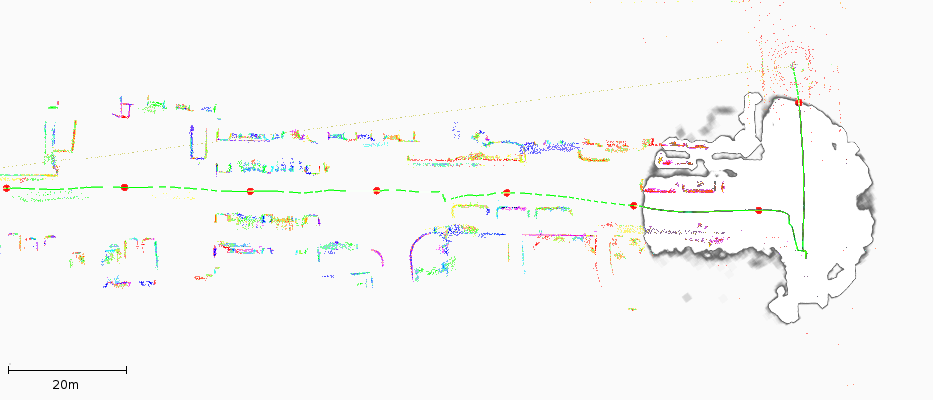
\includegraphics[width=5.2in]{images/seg_queue.png}
  \caption{The segmentation queue. Collectors shown in red, with the latest local map filtered to a cylinder visible at the right.}
  \label{fig:seg-queue}
\end{figure}

Fig.~\ref{fig:seg-queue} illustrates the process of online segmentation described above.
\subsection{Filtering Segments}

\label{subsec:filtering-segments}

\subsubsection{Sliced Segments}
\label{subsub:sec:sliced}

In the case where the SegMatch algorithm is applied to point clouds which have had a boundary filter applied, it is recommended to filter out segments which are partial views of objects split at the boundary.\\

These partial segments can lower the quality of the matches and of the general algorithm.\\

In order to do so, our method consists in first segmenting the boundary filtered point cloud, then applying a stricter version of the same boundary filter.\\

For example, say that the boundary filter is cylindrical of radius $R$. We only keep segments which do not spill outside of a smaller radius $r = R-b$, $b$ being the thickness of the outer zone. Segments that have points within this zone are considered to likely also possess points outside of $R$, and to therefore be sliced.\\

\subsubsection{Duplicates}
\label{subsub:sec:duplicates}

In our experiments, results indicate that it is necessary to prevent duplicate segments from being stored, as they later create duplicate matches.\\ 

These duplicate matches are detrimental to the Geometrical Clustering step, either artificially increasing the amount of matches in a cluster, or even creating clusters consisting only of identical matches ( with an exagerated transformation, since there is not enough true degree of freedom information in those duplicate matches ).


\section{Results}
\label{sec:segmatch-results}

\subsection{Influence of parameters}

This subsection evaluates the influence of algorithm parameters on the output.\\
%TODO

\subsection{Loop closures}

We were able to demonstrate loop closure capabilities with SegMatch, with minimal parameter tuning.
%TODO

\begin{figure}
  \centering
  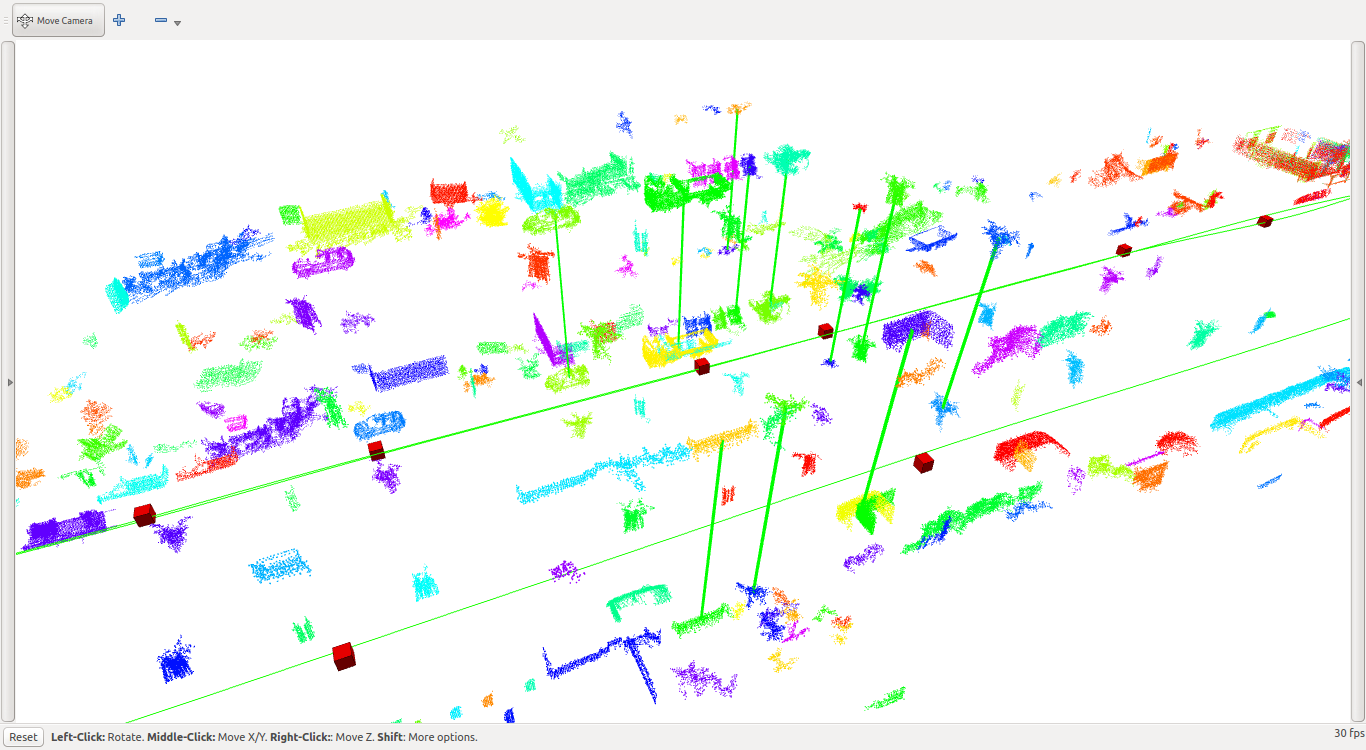
\includegraphics[width=5.2in]{images/segmatchae.png}
  \caption{Successful SegMatch loop closure detection on KITTI drive 20.}
  \label{fig:segmatch-loop-closure}
\end{figure}

Fig.~\ref{fig:corrected}.\\

\begin{figure}[!tbp]
  \centering
  \begin{minipage}[b]{0.4\textwidth}
    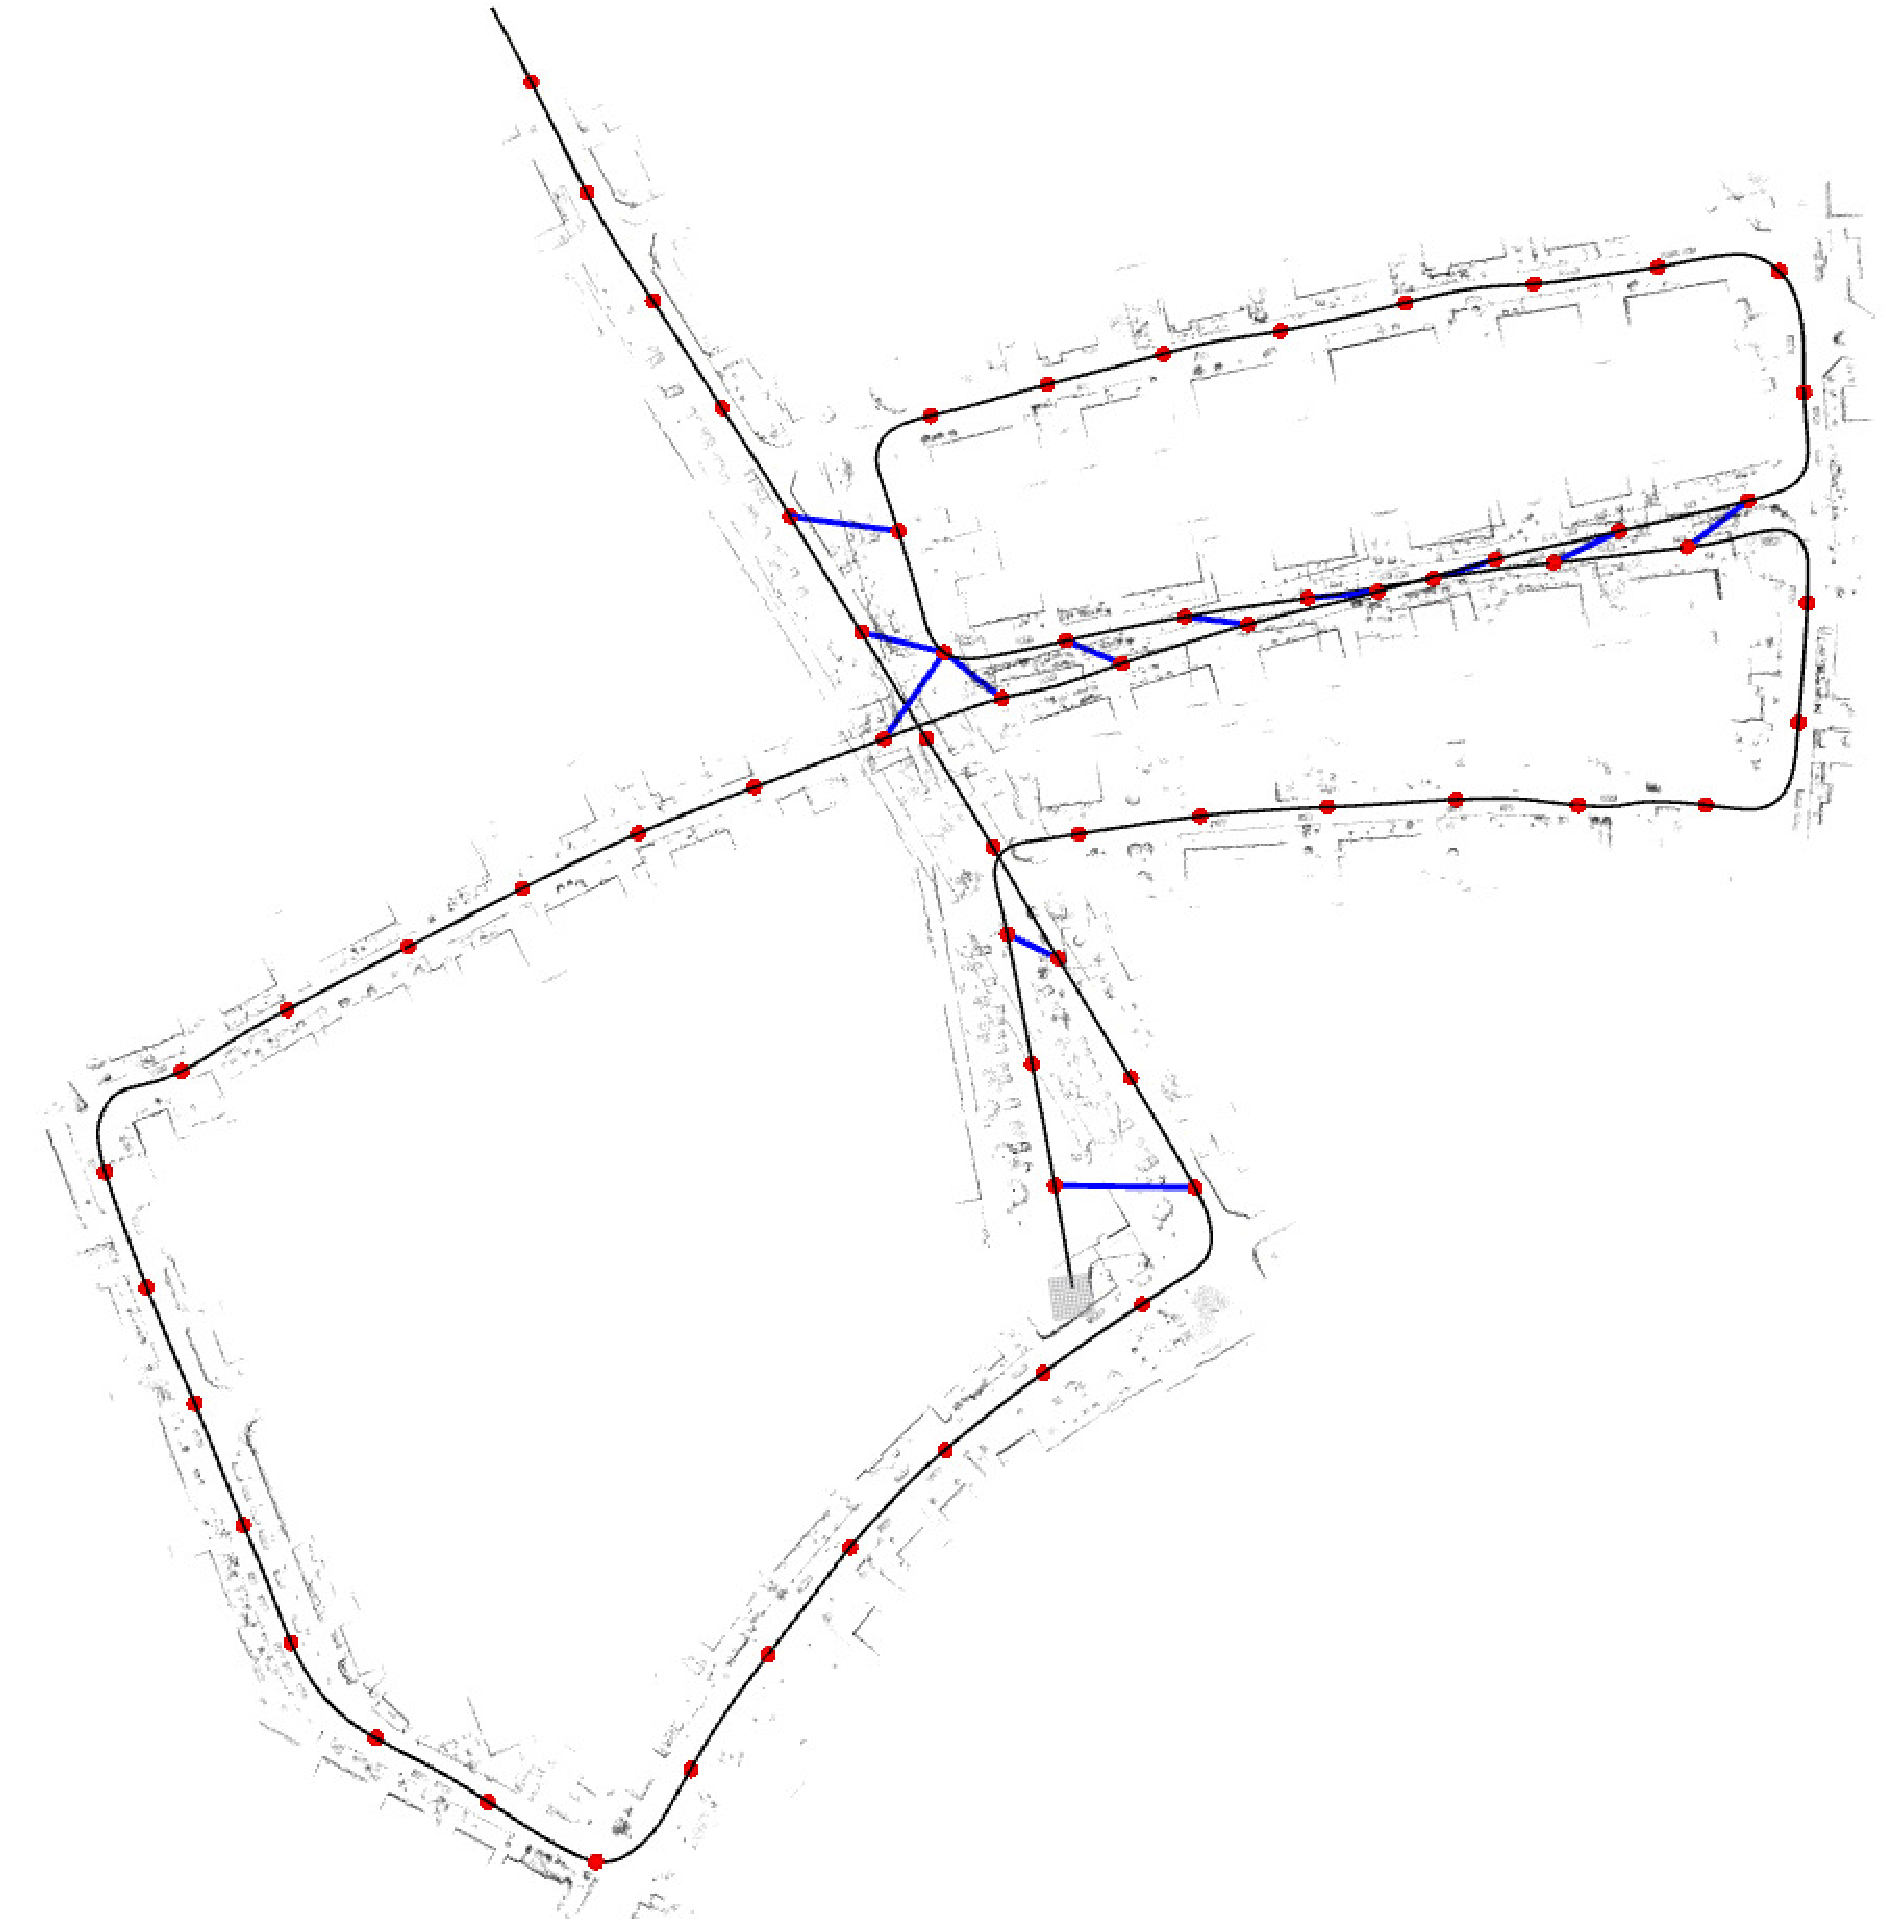
\includegraphics[width=\textwidth]{images/before_segmatch.pdf}
  \end{minipage}
  \hfill
  \begin{minipage}[b]{0.4\textwidth}
    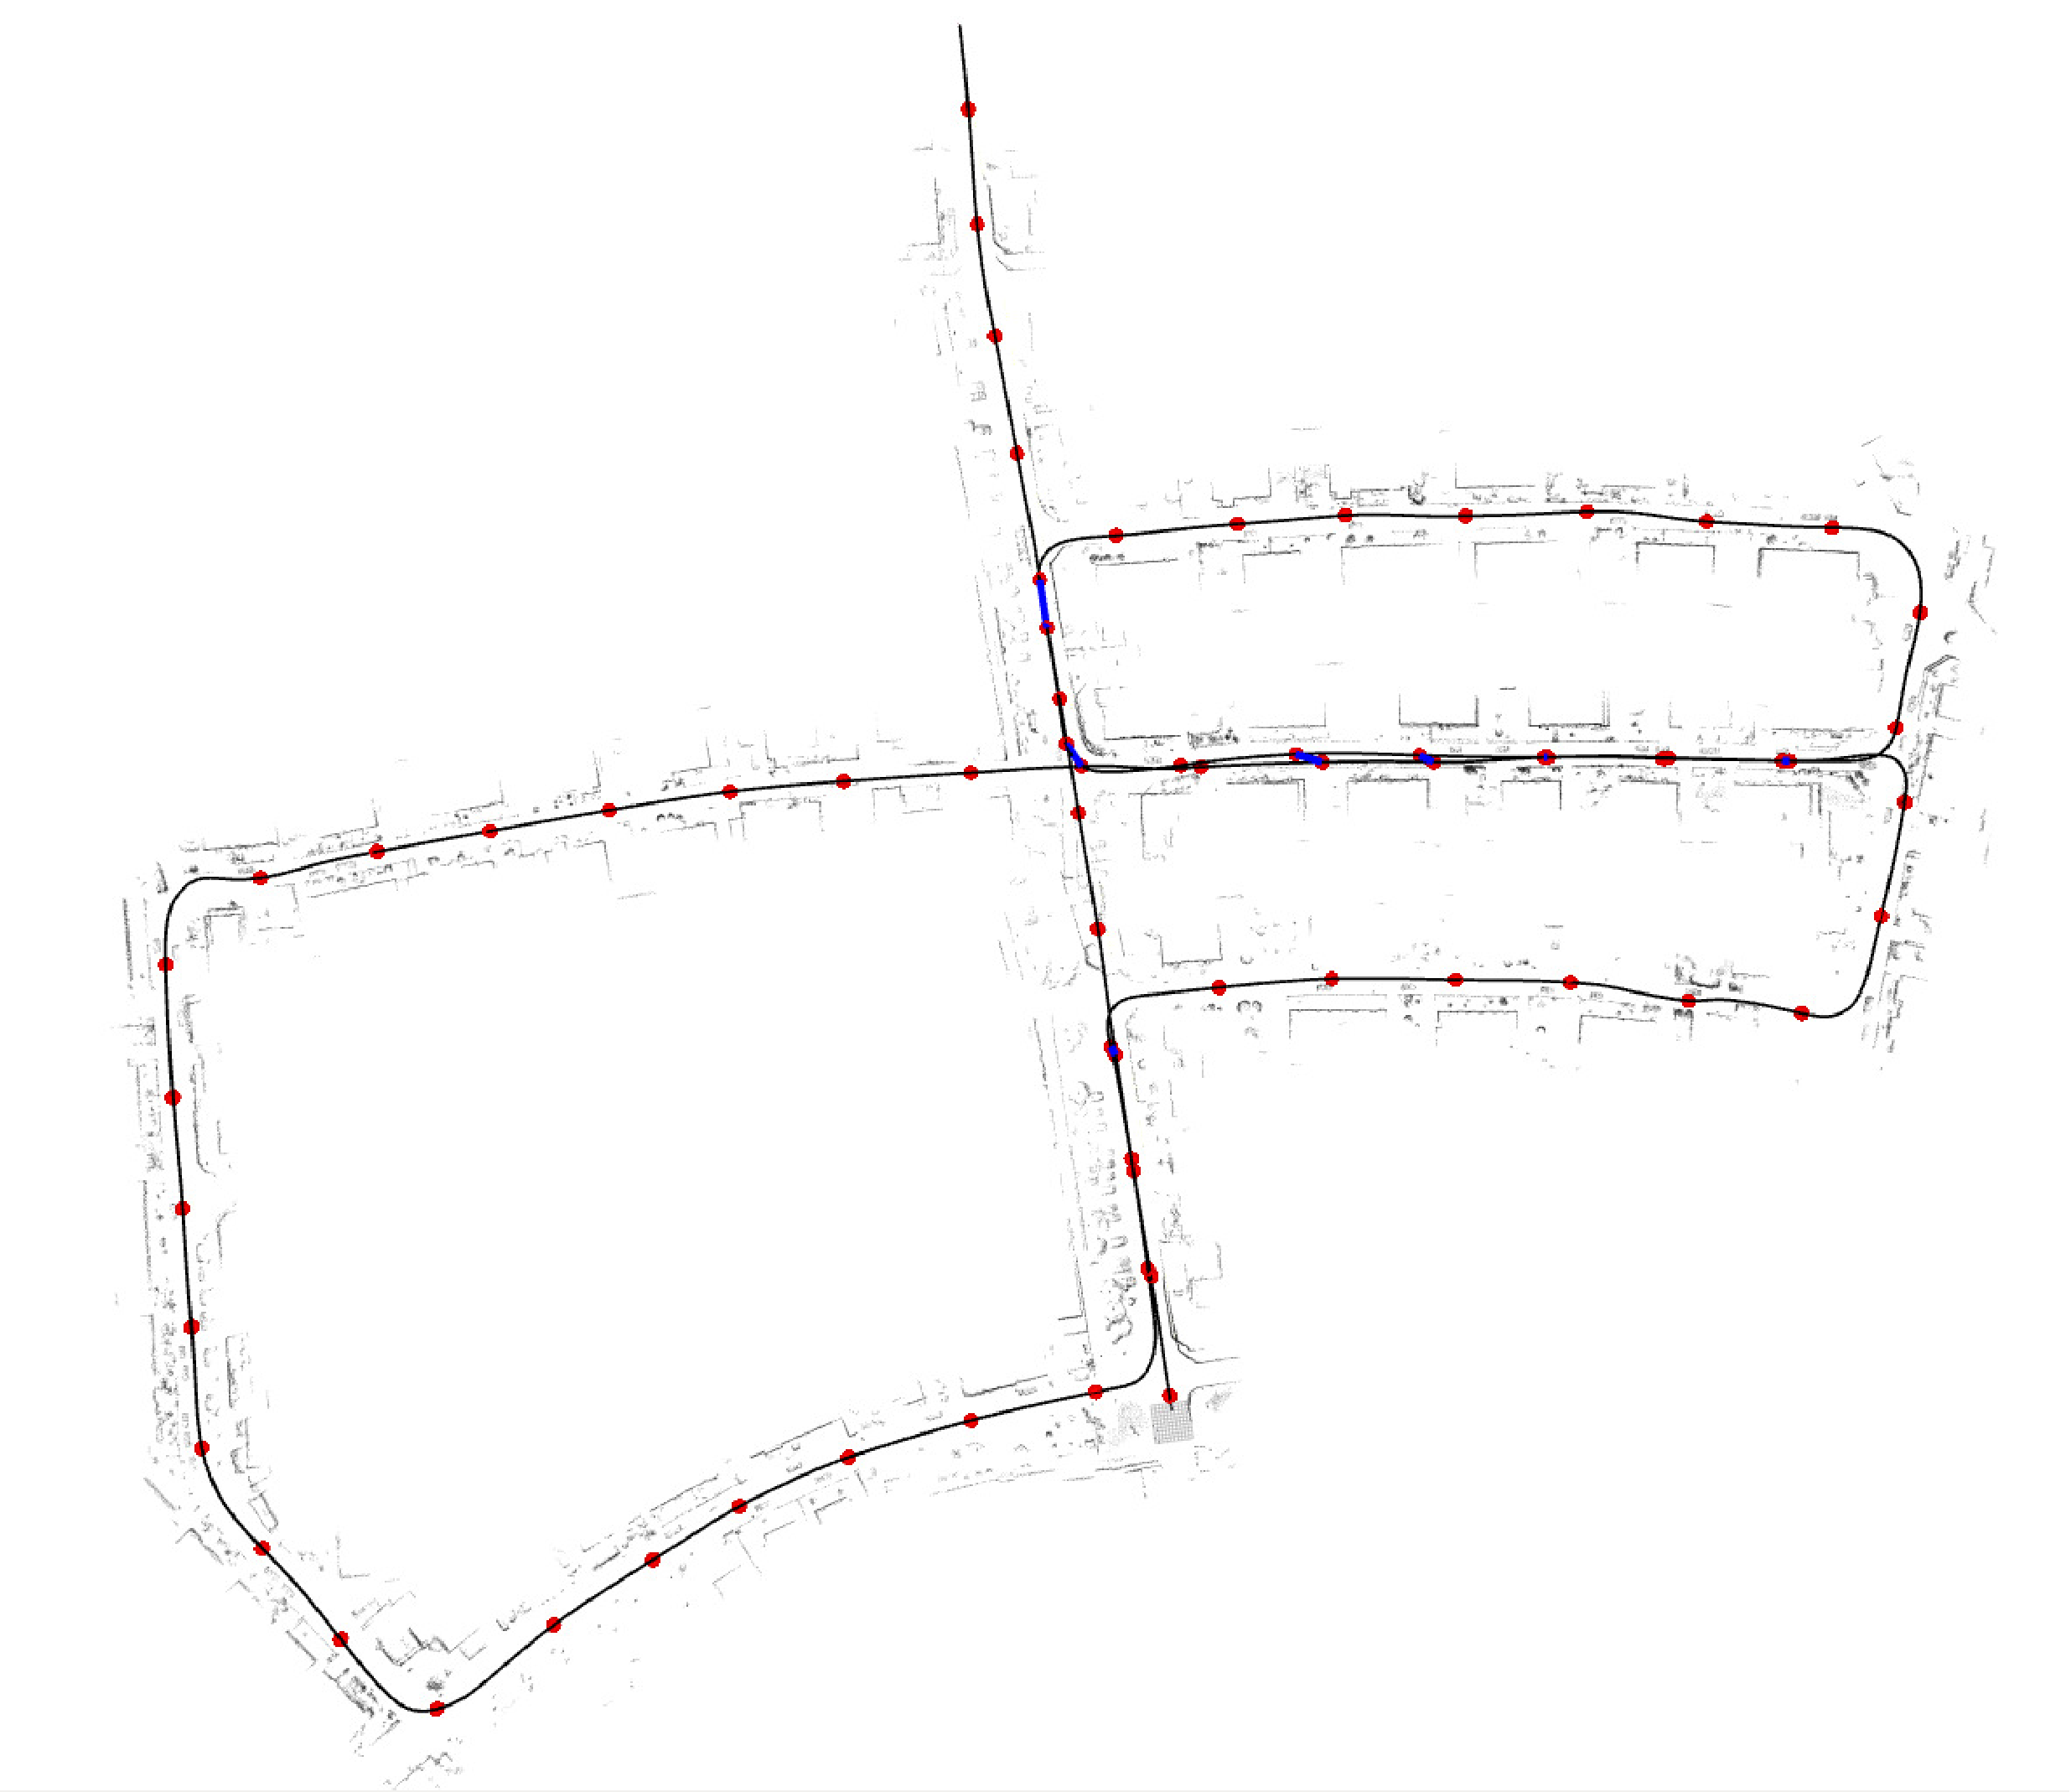
\includegraphics[width=\textwidth]{images/after_segmatch.pdf}
  \end{minipage}
  \caption{Recorded trajectory before (left) and after (right) being corrected with SegMatch loop closures. This image is taken from Dubé \cite{segmatch}}
  \label{fig:corrected}
\end{figure}

